\chapter{テトリスのカーソルを作る}
\section{カーソルの設計}
\subsection{カーソルの機能を考える}
カーソルというと、パソコンの矢印のことを思い浮かべるかもしれませんが、現在の
場所を示すものを指します。今回は、テトリスのカーソルを作ります。カーソルはどんな
変数・関数を持つといいでしょうか?今回も教科書の方で決めさせてもらいました。
\begin{itemize}
  \item カーソルの位置を表す変数2つ
  \item カーソルを上下左右に動かす関数
  \item カーソルを描画する関数
\end{itemize}
今回はカーソルのある列は灰色にすることにします。また、カーソルが盤面からはみ出さないように
する機能も上下左右に動かす関数が持つことにします
\footnote{こういう処理をmain関数とかにやらせてしまうと「良くない設計」と言われかねません。
  プログラマの中には「間違った設計」を見るとすごい勢いで設計について語り出す熱心な人もいます。そうした人にも一目置かれるようなプログラマを目指したいですね。}。
\subsection{カーソルの設計について考える}
「カーソルを描画する関数」とありますが、カーソルを描画する方法は2つあります。
\begin{itemize}
  \item カーソルがscreenに対して描画する
  \item カーソルがBoardに指令を出し、Boardがscreenに描画する
\end{itemize}
これらの方法について考えてみましょう。どちらがいいでしょうか?
\newpage
\subsection{設計にけりをつける}
\subsubsection{カーソルがscreenに対して描画する派の主張}
\begin{itemize}
  \item カーソルはBoardとは別の要素なので別に仕事を行うべき
  \item カーソルの情報を盤面に書き込むには、カーソルが盤面の情報にアクセスする必要があり、設計が増える
\end{itemize}
1つ目の要素については個人の自由なのでどちらでもいいですが、
2つ目の要素は考慮する必要があります。

\subsubsection{カーソルがBoardに指令を出し、Boardがscreenに描画する派の主張}
\begin{itemize}
  \item カーソルもBoardの一部
  \item screenに描画するクラスは一つにまとめた方がいい。Cursorもscreenにアクセスするべきではない。
\end{itemize}
実際、カーソルが盤面の一部かどうかについては、\textbf{人によります}。
でも、2つ目の要素は重要です。screenに描画するクラスは一つにまとめた方がいいです。
screenに関してバグがあった時に、screenにアクセスするクラスが一つにまとまっていると
バグの原因を特定しやすくなります。

\subsection{決着}
今回は、このようにします。
\begin{itemize}
  \item カーソルはBoardの一部
  \item カーソルは描画を\textbf{行わない}
\end{itemize}
なので、それぞれのクラスの中身を以下のように変更します。
\subsubsection{Boardクラス}
\begin{itemize}
  \item 盤面のブロックサイズを表す変数
  \item 盤面のブロックの状態を表すリスト
  \item カーソルを表す変数
  \item 盤面, \textbf{カーソル}をスクリーンに描画する関数
  \item 盤面のブロックサイズから画面の大きさを計算する関数
\end{itemize}

\subsubsection{Cursorクラス}
\begin{itemize}
  \item カーソルの位置を表す変数2つ
  \item カーソルを上下左右に動かす関数
\end{itemize}

\section{Cursorクラスを定義する}
\subsection{Cursorクラスを定義する}
tetris.pyにCursorクラスを追加します。
初期状態は中央上側にカーソルがある必要があるので、\_\_init\_\_関数で初期位置を設定します。
\lstinputlisting[title={Cursorクラスを作る}, language=Python]{chapter5/tetris.py}
これだとBoardに直接変数を追加しても良さそうな気もしますが、別の機能は別のクラスに書く、を徹底しましょう。
Boardクラスの\_\_init\_\_関数に「self.cursor = Cursor()」を追加していること、draw関数の最後に
「カーソルの列に対し、BLACKのマスをGRAYにする」処理を入れていることに注意してください。
main関数は変更しなくて大丈夫です。処理を任せることで変更部分を減らすことができるのもオブジェクト指向の特徴です。
実行するとカーソルが出るはずです。

\begin{figure}[h]
  \centering
  % 824x1600
  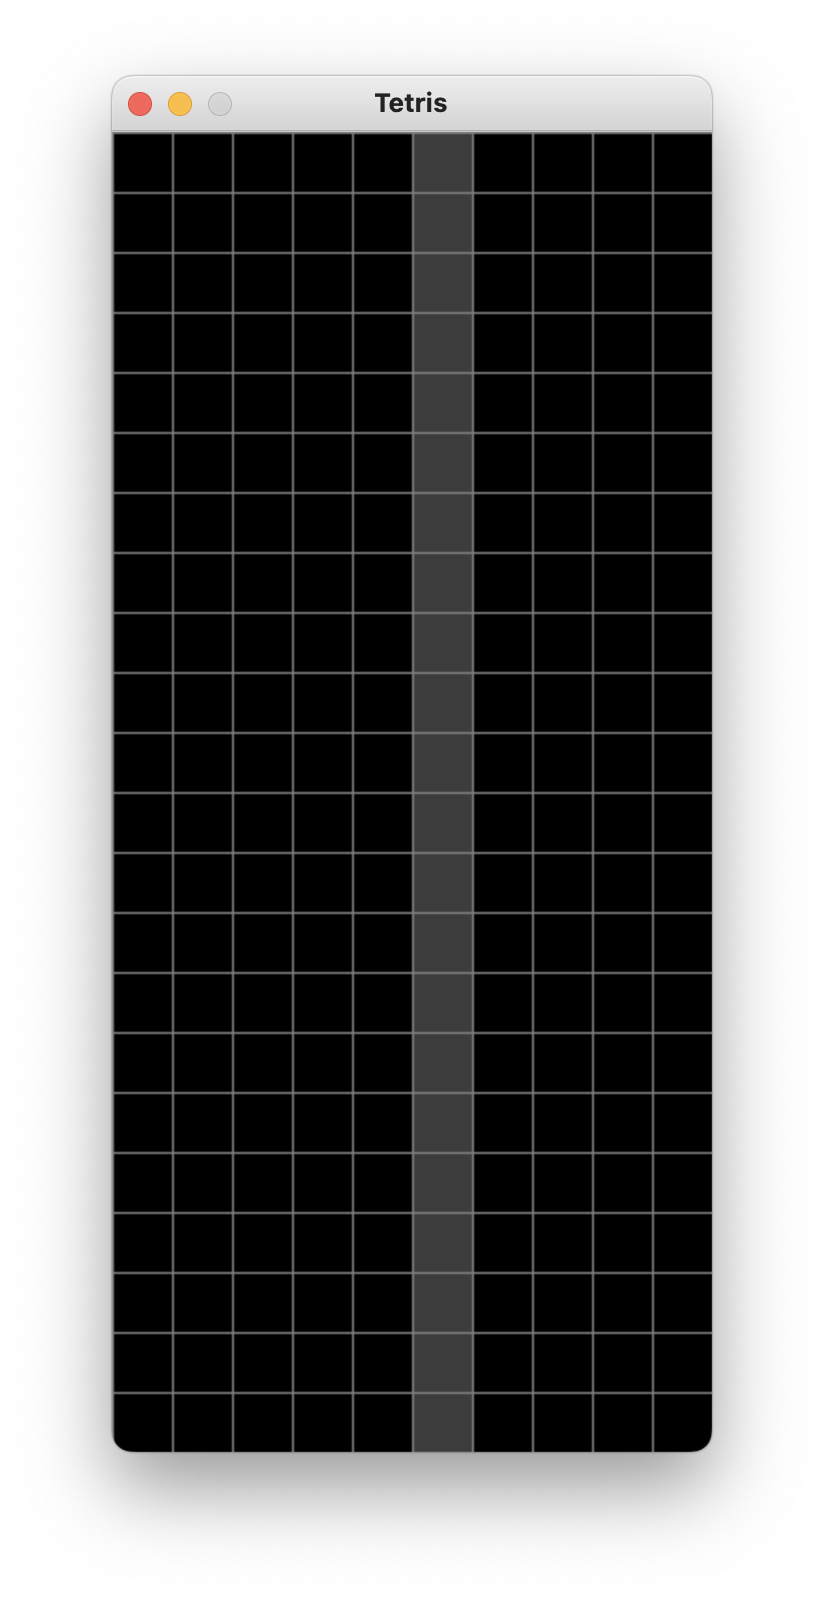
\includegraphics[height=15cm, natwidth=824,natheight=1600]{images/TetrisCH5.png}
  \caption{テトリスの実行結果}
\end{figure}

\section{カーソルを動かす}
\subsection{キー入力を受け取る}
カーソルを動かすには、キー入力を受け取る必要があります。
さて、画面の話でもありましたが、キー入力を受け取る存在も一つにまとめた方がいいです。
どうやって設計すればいいでしょうか?
\begin{itemize}
  \item キー入力を受け取るクラスを作る
  \item main関数にキー入力を受け取る処理を書く
  \item Boardにキー入力を受け取る処理を書く
  \item Cursorにキー入力を受け取る処理を書く
\end{itemize}
このような方法が浮かんできたら、あなたもオブジェクト指向プログラマーの仲間入りです。

キーを受け取るクラスを作る方法はとても「アリ」なんですが、今回はキーの数が少ないのでしません。
Boardにキー入力を受け取る処理を書くと、Boardがキー入力を受け取るという役割が増えてしまいますし、
そもそも盤面に対してキーを打っているわけではないので、これは残念ながら良くないデザインとされます。
Cursorも同様です。今回は「キー入力を受け取るのはmain関数の仕事」とします。後々一時停止や終了などのキーを
作った時に、それをカーソルが受け取るのは不自然ですよね。

\subsection{main関数でキー入力を受け取る}
先ほど決めた通り、main関数でキー入力を受け取ることにします。
\lstinputlisting[title={main関数でキー入力を受け取る}, language=Python]{chapter5/main2.py}
矢印キーでカーソルを動かせるようになりました。pygame.time.wait(100)という見慣れない
文があるかもしれませんが、これは100ミリ秒待つという意味です。mb.sleepと似ていますね。

\section{まとめ}
いろいろ考えた結果、今回はカーソルはBoardの一部ということにして、カーソルの描画はBoardに任せることにしました。
さらに、キー入力を受け取るクラスを作ることも考えましたが、今回はmain関数で受け取ることにしました。
このような設計は先を見据えて行うことが重要ですが、慣れないうちは「とりあえず動くもの」を作ることも大事です
\footnote{今回の設計も正しいとは言い切れません。Boardクラスが「Blob(ブロブ)」状態に陥る兆しがあります。詳しく知りたい人は調べたり聞いてみたりしてください。}。

\subsubsection{先生と考えよう}
キー入力を受け取るクラスを作る場合、どのような設計になるでしょうか?